\documentclass[12pt]{article}

\usepackage[hmargin=1in,vmargin=1in]{geometry}
\usepackage{parskip}
\usepackage{hyperref}
\usepackage{graphicx}
\usepackage{color}
\usepackage{verbatim}
\hypersetup{pdfstartview=FitV,hidelinks}



\begin{document}

{
  \Large
  \centering
  {\bf Lab 11 -- Estimating survival, recruitment, and growth rate
    with capture-mark-recapture data} \\
  Due before your next lab \par
}

\vspace{10pt}

% Analysis of the (fake) Mongolian gazelle ({\it Procapra gutturosa})
% data using program DISTANCE.

The purpose of this lab is to learn how to use program MARK to
estimate survival, recruitment, and growth rate using mark-recapture
data. Put your answers in a Word file named something like
``Chandler-lab10.docx'', and upload it to ELC.




%\clearpage

\section*{\large Exercise I: }


\clearpage

\section*{\large  Exercise II: The Jolly-Seber model for estimating
  survival, recruitment, and growth rate}

{\bf Instructions}

\begin{enumerate}
  \item Create a New Project, name it \verb+"Exercise II"+, and select
    the \verb+"CH-SO-Dean-AllYears.inp"+ data file.
  \item Choose the \verb+"Jolly-Seber"+ Data Type
  \item Set \verb+"Encounter Occasions"+ to 6 (for 6 years of data)
  \item Sampling occurred on years 2007, 2010, 2011, 2012, 2014, and
    2015, so the time interval among sampling occasions differs. To
    account for this, select \verb+"Set Time Intervals"+ and specify the
    time gaps as 3, 1, 1, 2, 1. Hit \verb+"OK"+, then hit it again on
    the next screen.
  \item Close the next screen and then click
    \verb+"PIM > Change Data Type"+ and select the
    \verb+"Link-Barker Jolly-Seber"+ option. This lets us estimate
    survival, recruitment, and p rather than survival, growth rate and
    p, which is the default option.
  \item Use the \verb+"Run > Pre-defined Model(s)"+ option to fit at
    least 3 different model. Basically, you can let each parameter be
    constant or allow it to vary among years, the \verb+"(t)"+ option.
  \item Right-click on the model with the lowest AICc
  score and selected \verb+"Derived parameters"+ to view yearly
  estimates of lambda.
\end{enumerate}


% \begin{figure}[h!]
%   \centering
%   \fbox{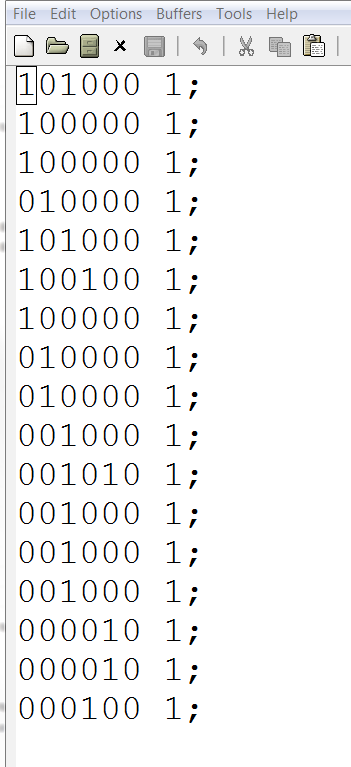
\includegraphics[height=7.5cm]{figs/stinkpot07-data}}
%   \caption{\small Stinkpot capture histories in a text file ready to
%     be imported to MARK.}
%   \label{fig:stink07-data}
% \end{figure}

{\bf Questions}

\begin{enumerate}
  \item What model is the best in terms of AICc?
  \item Interpret the parameter estimates from the model with the
    lowest AICc. (For parameters that are year-specific, you do not
    need to interpret each yearly-estimate.)
  \item What are the estimates of lambda for each time interval? These
    can be found by right-clicking on a model and choosing
    \verb+"Derived parameters"+.
  \item What is the relationship between the estimates of survival,
    recruitment and lambda?
  \item Bring the estimates of lambda into Excel and create a plot of
    lambda over time.
  \item What conclusions about this population would you draw from
    this analysis? Do you think it is growing, shrinking, remaining
    constant, or is it difficult to tell?
  \item How could you get more precise parameter estimates?
\end{enumerate}

\begin{table}[h!]
  \centering
  \caption{A description of the four models to be fitted to the
    stinkpot data.}
  \footnotesize
  \begin{tabular}[h!]{ll}
    \hline
    Model name & Model description \\
    \hline
    $M_0$ & The most basic model in which $p$ and $c$ are constant \\
    $M_t$ & A model in which $p$ differs among sampling occasions and
            $p_t=c_t$. \\
    $M_b$ & A behavioral response model in which $p$ and $c$
            differ. Can describe trap happiness or trap shiness. \\
    $M_{tb}$ & A combination of models $M_t$ and $M_b$. \\
    \hline
  \end{tabular}
  \label{tab:Otis}
\end{table}




{\bf Parameter definitions}
\begin{itemize}
  \item $p$ -- capture probability. The probability of capturing an
    individual on a single occasion
  \item $p_t$ -- capture probability on occasion $t$
  \item $c$ -- recapture probability. The probability of capturing an
    individual that has been captured previously.
  \item $n$ -- the number of individuals captured
  \item $f_0$ -- the number of individual not captured
  \item $N$ -- abundance. The number of individuals in the
    population. $N=n+f_0$.
\end{itemize}






\end{document}




